
Our overview of the argument follows the exposition of \cite{MR2528734}, which in turn outlines the stability result for $m \geq 4$ in \cite{gustafson2007schrodinger}; we will leave the modifications of the argument in \cite{GustafsonEtAl2010} to handle the $m = 3$ case to the details. For our notation, we will instead borrow from \cite[Geometric Wave Equations]{KochEtAl2014} and \cite{BejenaruTataru2014,bejenaru2024near}. 

We decompose the solution into a soliton profile and a dispersive error,
\begin{equation}\label{eq:decomp2}
	u(t, r) = \underbrace{Q_{\alpha(t), \lambda(t)}(r)}_{\text{modulated soliton}}  + \underbrace{\epsilon(t, r)}_{\text{dispersive error}} .
\end{equation}
To prove the main theorem, we want construct appropriate modulation parameters $(\alpha, \lambda)$ and correction term $\epsilon$ such that 
	\begin{enumerate}
		\item the error obeys global-in-time dispersive bounds, $\epsilon \in \mathsf S_{t, x}^1 ([0, \infty) \times \R^2)$, to obtain the dispersive decay, and \label{item:goal1}
		
		\item integrability bounds on the derivative of the modulation parameters, $(\dot {\alpha}, \dot{\lambda}) \in L^1_t ([0, \infty))$, to conclude convergence to a soliton. \label{item:goal2}
	\end{enumerate}
Here the $\mathsf S_{t, x}^1$-norm is taken to be a scale-invariant Strichartz-type norm at the level of the differentiated field $\partial u$. For our purposes, it will suffice to take the dispersive norm to consist of the endpoint norms, 
    \[
        ||\epsilon||_{\mathsf S_{t, x}^1} 
            := ||\epsilon||_{L^\infty_t \dot H^1_x} + || r^{-1}\epsilon ||_{L^2_t L^\infty_x}. 
    \]

\subsection{Generalised Hasimoto transformation}
	Generally, one would have to study the dynamics of the error coupled with the dynamics of the modulation parameters. However, the Schr\"odinger maps equation \eqref{schrodinger} admits \textit{self-dual} structure, which we first saw from the Bogomoln'yi identity \eqref{B}. Viewing the Schr\"odinger maps equation as the Hamiltonian flow of the Dirichlet energy, the Bogomoln'yi identity implies that the equation can be written as  
	\begin{equation}\label{eq:selfdual}
		\begin{split}
			\partial_t u 
				&= \bfJ \bfD_z \partial_{\overline z} u,
		\end{split}
	\end{equation}
    where 
    \begin{align*}
        \partial_{\overline z} u  
            &:= \partial_1 u - \bfJ \partial_2 u ,\\
        \bfD_z v 
            &:= \bfD_1 v + \bfJ \bfD_2 v. 
    \end{align*}
Then, applying the covariant Cauchy-Riemann operator to the self-dual formuation \eqref{selfdual}, we obtain the generalised Hasimoto-transformed Schr\"odinger maps equation, which is an elliptic-dispersive system,
    \begin{align}
        \bfD_t \epsilon'
            &= \bfJ \bfD_{\overline z} \bfD_z \epsilon' \label{eq:hasimoto2},\\
        \epsilon'
            &= \partial_{\overline z} u . \label{eq:hasimoto3}
    \end{align}
This is known as the \textit{generalised Hasimoto transformation}\footnote{The original Hasimoto transformation was derived in the context of fluids mechanics to transform the vortex filament equation into the one-dimensional cubic non-linear Schr\"odinger equation. The one-dimensional Schr\"odinger maps arises as the equation for the unit tangent field to the vortex filament. We point the interested reader to the classical book of Majda-Bertozzi \cite[Chapter 7.1]{MajdaBertozzi2002} for details. 
}, derived originally by Chang-Shatah-Uhlenbeck in \cite{ChangEtAl2000}. 
This formulation is convenient for two general reasons (see \cite[Chapter 6.2]{Tao2006} and \cite[Chapter 2.5]{KochEtAl2014} for more commentary on the \textit{frame method}) and one particular to the self-dual structure: 
    \begin{enumerate}
        \item the differentiated field takes values in a vector bundle $\epsilon' : I \times \R^2 \to u^* T \SS^2$ rather than a manifold like the original field $u: I \times \R^2 \to \SS^2$, so one can work in linear function spaces,
        
        \item we are free to choose an orthonormal frame for the bundle $u^* T\SS^2$ to concoct a favourable equation for $\epsilon'$ in coordinates, 
        
        \item in view of the harmonic maps equation \eqref{CR}, one can think of the map $u \mapsto \epsilon'$ as a non-linear projection which kills the harmonic maps component, leaving only the error, i.e. the differentiated field is at least linear in the error 
            \[
                \epsilon' = O(\epsilon) + O(\epsilon^2).
            \] 
        Thus we can view \eqref{hasimoto2} as a small $L^2_x$-data problem for a Schr\"odinger equation with cubic non-linear interactions. Using standard Strichartz estimates, it is well known that solutions to such equations admit global-in-time dispersive bounds $\epsilon' \in \mathsf S_{t, x}^0 ([0, \infty) \times \R^2)$. 
    \end{enumerate}
Our strategy then will be to prove dispersive estimates for the differentiated variable $\epsilon'$ using the non-linear Schr\"odinger equation \eqref{hasimoto2}. Using elliptic estimates for the inhomogeneous Cauchy-Riemann equation \eqref{hasimoto3}, we can pass these dispersive decay estimates onto the original error $\epsilon$. 
    \[
        ||\epsilon'||_{\mathsf S_{t, x}}
            := ||\epsilon'||_{L^\infty_t L^2_x} + || \epsilon'||_{L^2_t L^\infty_x}
    \]





\subsection{Orthogonality and modulation}

To identify the main enemy to proving decay estimates for the error, let us consider the linearisations of the Schr\"odinger maps equation \eqref{selfdual} and the Cauchy-Riemann equation \eqref{hasimoto3} about a fixed soliton profile $Q$. A solution to the linear flow is a field $u_{\mathrm{lin}} : I \times \R^2 \to Q^* T\SS^2$, which, upon choosing appropriate coordinates, e.g. Coulomb gauge $\{\vec v_Q, \vec w_Q \} \subseteq Q^* T\SS^2$, corresponds to a complex scalar field $\phi_{\mathrm{lin}} : I \times \R^2 \to \C$ satisfying 
    \begin{align}
        (i \partial_t - \mathsf{H}_Q) \phi_{\mathrm{lin}} \label{eq:linearised}
        &= N,\\
    \mathsf L_Q \phi_{\mathrm{lin}}
        &= F,\label{eq:linearisedCR}
    \end{align}
where $\mathsf H_Q$ is the \textit{linearised operator} and $\mathsf L_Q$ is the \textit{linearised Cauchy-Riemann operator}, given by 
\[
    \mathsf{H}_Q 
        := \mathsf{L}_Q^* \mathsf{L}_Q, 
        \qquad 
    \mathsf{L}_Q 
        := h_1 \partial_r {h_1}^{-1}.
\]
The factorisation of the linearised operator a l\'a the linearised Cauchy-Riemann operator can be read off from the self-dual structure of the equation. We see that the main enemy to decay of the error $\epsilon \approx \phi_{\mathrm{lin}}$, either via dispersive estimates from \eqref{linearised} or elliptic estimates from \eqref{linearisedCR}, would be the kernel of the linearised operators. From the perspective of the dispersive equation, the kernel elements lead to non-decaying, constant-in-time solutions, while from the perspective of the elliptic equation, the non-trivial kernel leads to non-uniqueness when attempting to invert the operator. 


\begin{figure}[h]\label{fig:orth}
    \begin{center}
        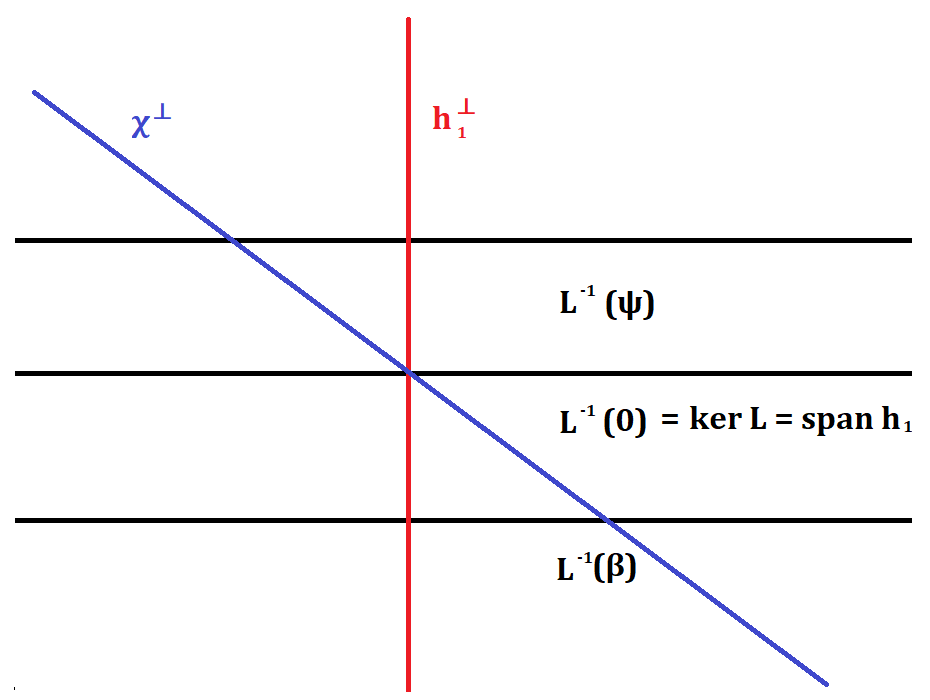
\includegraphics[scale = 0.4]{graphics/inverse}
        \caption{The level sets of the linear operator $\mathsf L_Q$ are affine subspaces of the domain which are parallel to the kernel 
            \[
            \mathsf L_Q^{-1} (\psi) = \phi + \ker \mathsf L_Q.
            \] 
        To identify a unique member $\phi$ in the level set, one must restrict the operator $\mathsf L_Q$ to a subspace which is transverse to the kernel. 
            }
    \end{center}    
\end{figure}

The kernel is given by 
\[
    \ker \mathsf{H}_Q = \ker \mathsf L_Q = \operatorname{span}_\C h_1.
\]
One can either read this off from the conjugation $\mathsf L_Q = h_1 \partial_r h_1^{-1}$ or invariance of the non-linear equations under scaling and rotation, which tells us that differentiating the modulated soliton $Q_{\alpha, \lambda}$ in these parameters generates elements of the kernel,
\begin{equation}\label{eq:generators}
    \begin{split}
    \frac{\partial Q_{\alpha, \lambda}}{\partial \alpha}\Big|_{(\alpha, \lambda) = (0, 1)}
        &= h_1 \vec v_Q,
        \\
    \frac{\partial Q_{\alpha, \lambda}}{\partial \lambda}\Big|_{(\alpha, \lambda) = (0, 1)} 
        &= h_1 
        \vec w_Q.
    \end{split}
\end{equation}

To kill these enemies, it will suffice to impose an orthogonality condition on the error, see Figure \ref{fig:orth}. 


Fix $\chi : (0, \infty ) \to (0, \infty)$ a radial, non-negative function which does not lie in the kernel, 
    \begin{equation}\label{eq:orthogonal1}
        \big\langle \epsilon, \chi^\lambda \big\rangle_{L^2_x} 
            = 0.
    \end{equation}
To enforce the orthogonality condition for all time, it suffices to solve the ODE furnished by differentiating the condition in time and imposing the condition holds initially at $t = 0$. This fixes the decomposition \eqref{decomp2}, as substituting it into the resulting ODE and using the equation \eqref{schrodinger} furnishes the \textit{modulation equation} for the parameters $(\alpha, \lambda)$. 

The linearised equations motivate two goals of the decomposition \eqref{decomp2},
\begin{enumerate}
    \item respects the linear flow \eqref{linearised},
    \item good elliptic estimates for the linearised Cauchy-Riemann operator \eqref{linearisedCR}. 
\end{enumerate}
Our first take would be to impose the condition that the error "$\epsilon \approx \phi$" is orthogonal to the kernel of the linearised operator $\mathsf H_Q$, 
\begin{equation}\label{eq:orthogonal}
    \phi_{\mathrm{lin}} \perp \ker \mathsf{H_Q} \qquad \text{"i.e."} \qquad \int_0^\infty \phi_{\mathrm{lin}} \, \overline{h_1} \, r dr 
        = 0. 
\end{equation}
This is a decomposition\footnote{Since the error is in the energy space, $\epsilon \in \dot H^1_m (\R^2)$, the orthogonality condition on the right is well-defined provided that $rh_1 \in L^2_r ([0, \infty))$ by Cauchy-Schwartz. The spatial asymptotics of the kernel elements are precisely $h_1 (r) = O(r^{-m})$, so one must restrict to the high equivariance case $m \geq 3$ to make sense of the orthogonality condition. } into invariant subspaces of the linearised flow, 
\[
    L^2_r ([0, \infty)) = \ker \mathsf H_Q \oplus (\ker \mathsf H_Q)^\perp.
\]
In view of the orthogonality of the error \eqref{orthogonal} to the generators of the kernel \eqref{generators}, the forcing terms in the modulation equations which are \textit{linear} in the error $\epsilon$ are killed, so
the derivatives of the parameters $(\dot{\alpha}, \dot{\lambda})$ only see \textit{quadratic} forcing terms and higher,
\begin{equation}\label{eq:quadratic}
    |\dot \alpha| + |\dot{\lambda}| 
        = O(|\epsilon|^2). 
\end{equation}
Thus, ignoring any technical problems with spatial asymptotics of $\epsilon$, an $L^2_t$-dispersive estimate for $\epsilon$ would imply an $L^1_t$-estimate for the parameters. This is favourable from the perspective of dispersive estimates, since our earlier discussion gives us access to $L^2_t L^\infty_x$-bounds on the differentiated error $\epsilon'$. At the level of the linearised Cauchy-Riemann operator, we would like to invert the operator and prove the fixed-time estimate 
    \[
        || r^{-1}\phi ||_{L^\infty_x} 
            \lesssim ||\mathsf L_Q \phi||_{L^\infty_x}.
    \]
By duality, one necessarily needs to place the function we are projecting away from in the dual space, i.e. we need $r \chi \in L^1_x (\R^2)$. In view of the asymptotics $h_1 = O(r^{-m})$, one necessarly needs $m \geq 4$. To reach $m = 3$, we need to replace our orthogonality condition with a generic test function $\chi \in C^\infty_c (0, \infty)$; this price one pays is that the linearised flow \eqref{linearised} no longer preserves the decomposition, so $(\dot{\alpha}, \dot{\lambda})$ are forced by linear terms in $\epsilon$ in the modulation equations,
    \[
        |\dot{\alpha}| + |\dot{\lambda}| 
            = O(\epsilon) + O(\epsilon^2). 
    \]
To handle the linear terms, we make a \textit{normal form transformation}.




